\section{TAREA 1: IMPORTACION DE DATOS USANDO EL WIZARD – SQL MANAGMENT} 

\begin{enumerate}
    \item Crear una base de datos – BDTEST
        \begin{center}
             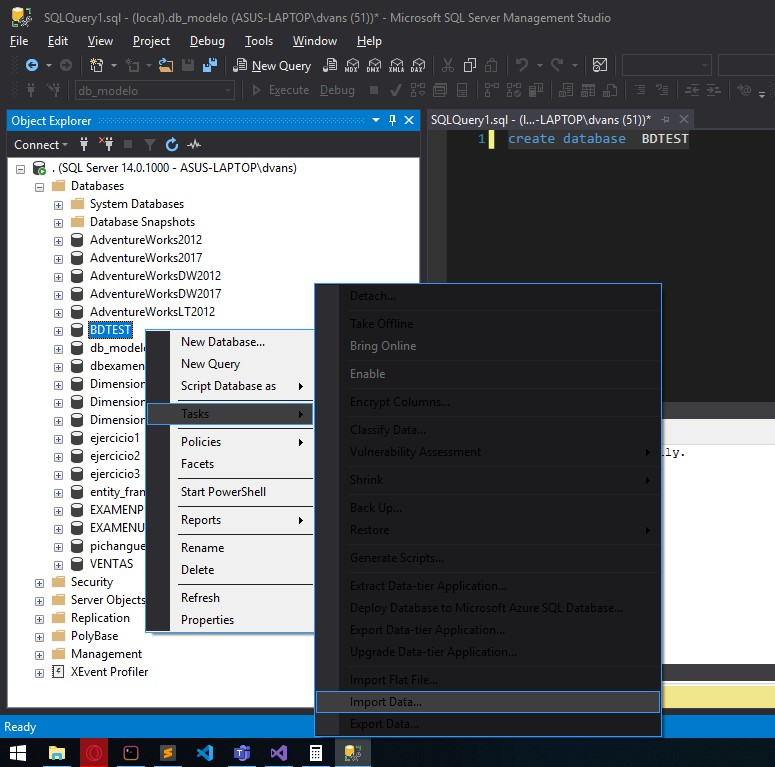
\includegraphics[width=10cm]{imagenes/importa_data_1.jpg}
        \end{center}
        
     \item Elegimos la base de datos origen
        \begin{center}
             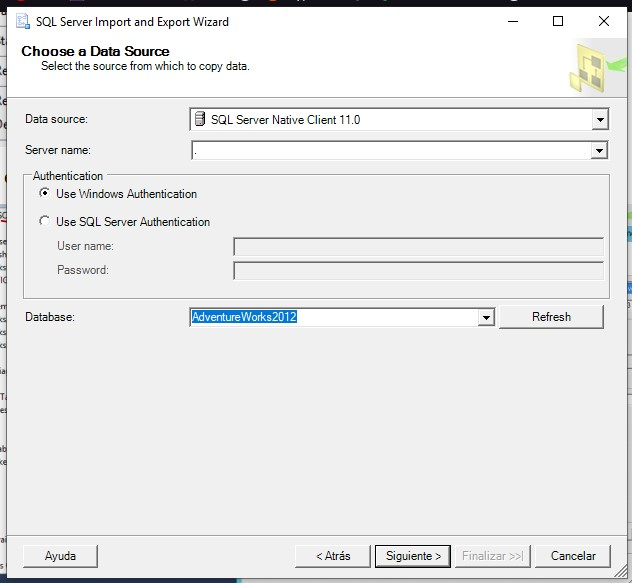
\includegraphics[width=10cm]{imagenes/importa_data_2.jpg}
        \end{center}
        
        \newpage
        
     \item Elegimos la base de datos destino
        \begin{center}
             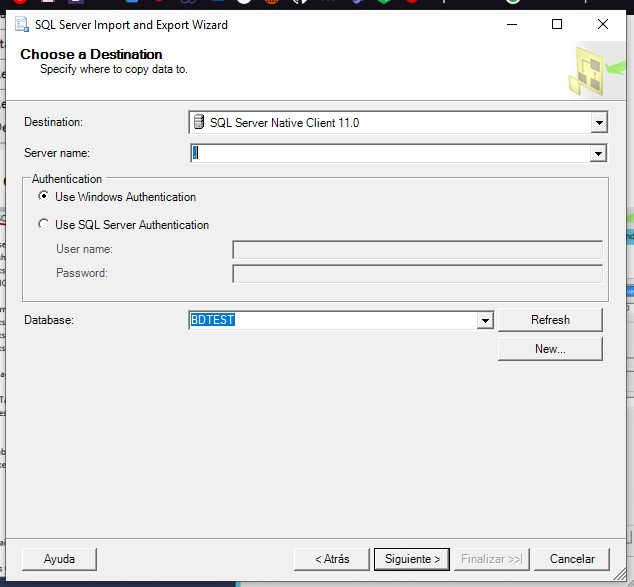
\includegraphics[width=10cm]{imagenes/importa_data_3.jpg}
        \end{center}
        
     \item Selecionamos la primera opcion
        \begin{center}
             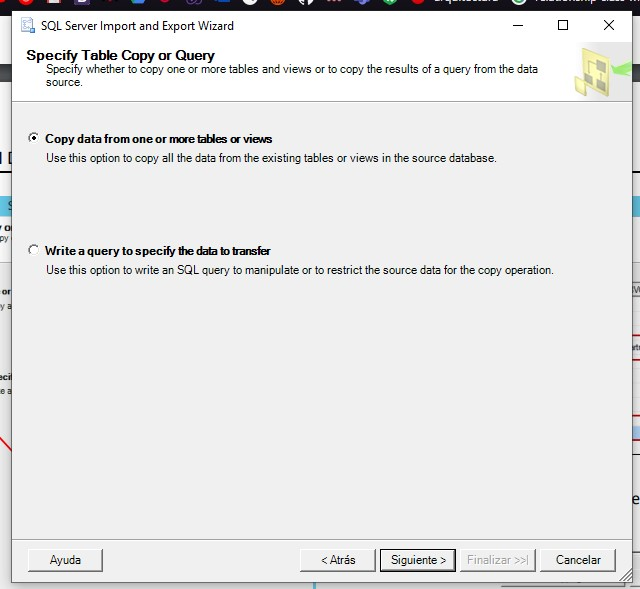
\includegraphics[width=10cm]{imagenes/importa_data_4.jpg}
        \end{center}
        \newpage
        
     \item Selecionamos las tablas Human.Deparment y Person.Address
        \begin{center}
             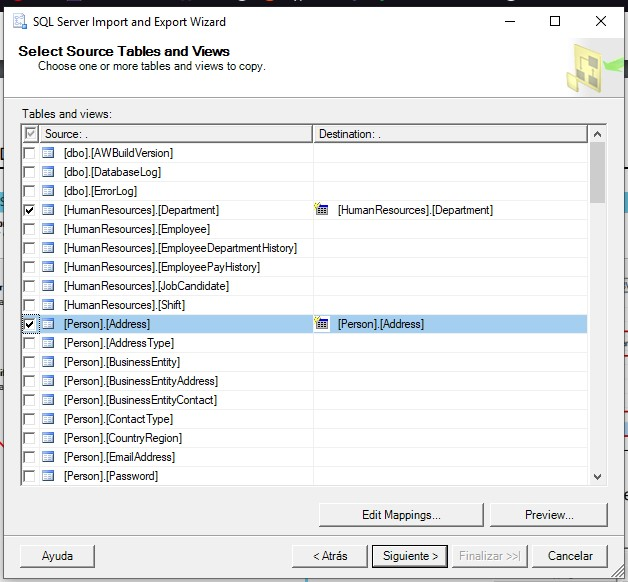
\includegraphics[width=10cm]{imagenes/importa_data_5.jpg}
        \end{center}
        
     \item Activamos para que guarde el paquete
        \begin{center}
             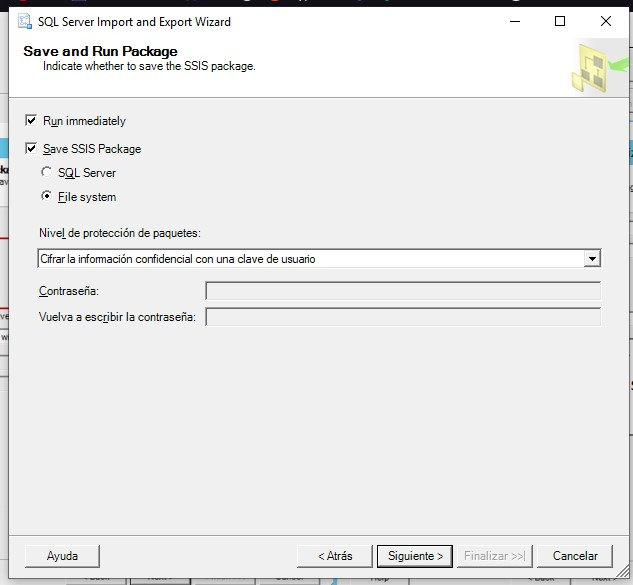
\includegraphics[width=10cm]{imagenes/importa_data_6.jpg}
        \end{center}
        \newpage
        
     \item Asignamos nombre y ruta del archivo
        \begin{center}
             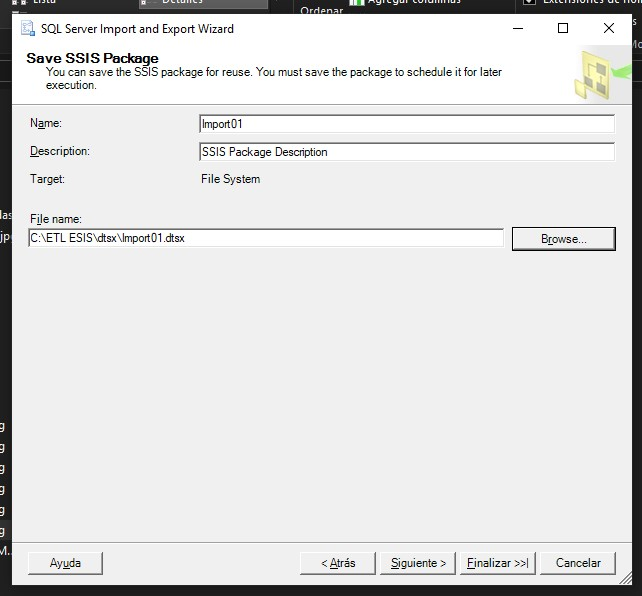
\includegraphics[width=10cm]{imagenes/importa_data_7.jpg}
        \end{center}
        
     \item Presionamos en finalizar
        \begin{center}
             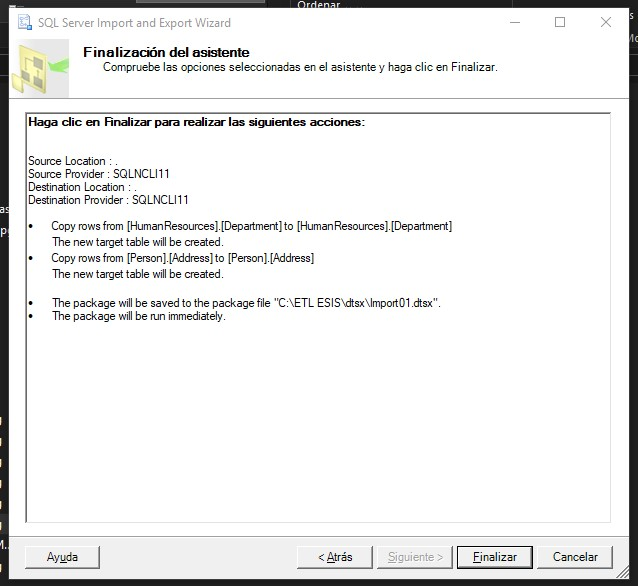
\includegraphics[width=10cm]{imagenes/importa_data_8.jpg}
        \end{center}
        \newpage
                
     \item Una vez terminado el procedimiento , presionamos en el boton Cerrar
        \begin{center}
             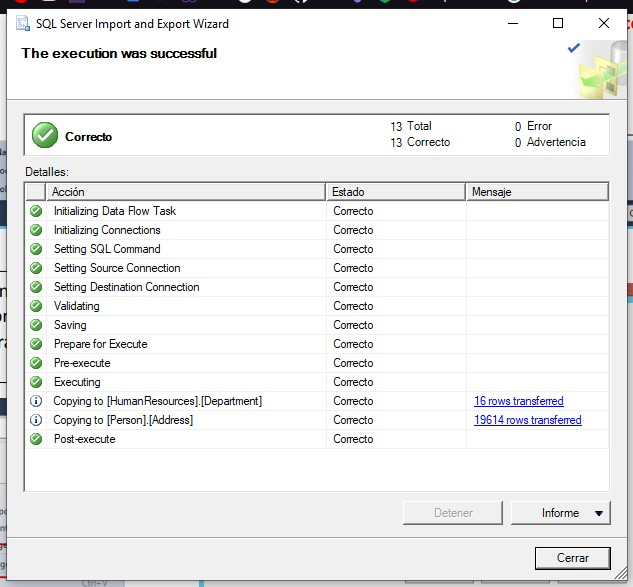
\includegraphics[width=10cm]{imagenes/importa_data_9.jpg}
        \end{center}

\end{enumerate}